\chapter{Practice: Wireless doorbell}\label{pract:wirelessDoorbell}
\section*{Suggested read: Chapters~\ref{introToXBee} and~\ref{pract:simpleChat}}

This practice guides you through the construction of a wireless doorbell system. It is composed by two components: the switch and the buzzer.

On the switch side, we will be prototyping a layout like the one shown in Figure~\ref{fig:wirelessDoorbellSwitch}. While the sound will be produced by a buzzer on the other radio, like in Figure~\ref{fig:wirelessDoorbellBuzzer}.

You will need:

\begin{itemize}
  \item Eventhough the two components may fit in one breadboard; to make it more real, it is better to use two separate breadboards.
  \item Hookup wire. It is recommended to have at least four different colors.
  \item Two Arduino boards.
  \item USB A-to-B cable for the Arduinos.
  \item One $10$K$\Omega$~resistor.
  \item One momentary switch or pushbutton for input.
  \item One buzzer for output.
  \item One XBee radio configured as \texttt{ZIGBEE COORDINATOR AT}.
  \item One XBee radio configured as \texttt{ZIGBEE ROUTER AT}.
  \item Two breakout boards.
  \item USB cable for the XBee breakout board.
\end{itemize}

Every ZigBee network has only one coordinator. Other nodes can be configured as routers. To configure your XBee radios, please refer to Chapter~\ref{xbeeRoleConfiguration}.

It is strongly suggested that you mark down the XBees to distinguish the coordinator from the router(s).

\section{Wireless doorbell connections layout}

\subsection{Switch}
Follow these guidelines to prepare the connections for the switch that will make the doorbell ring (or buzz in our case). If lost, you can always take a look at the final layout in Figure~\ref{fig:wirelessDoorbellSwitch}.

\begin{enumerate}
  \item Energize the breadboard by hooking up a {\color{red}{red}} wire from the Arduino $3.3$V output to one of the power rails of the breadboard.
  \item Hook up a {\color{blue}{blue}} wire from the ground (GND) connection on the Arduino to the ground rail on the breadboard.
  \item Place the XBee/breakout board with both sides on different sections of the breadboard, in a way that the space separating the sections passes under the XBee/breakout board.
  \item Use a {\color{red}{red}} wire to connect pin $3.3$V (or pin $1$ as in Figure~\ref{fig:xbeeBreakoutBoardPins}) of the XBee to the power rail on the breadboard.
  \item Use another color cable to hookup the XBee's GND pin to the ground in the breadboard.
  \item Grab another color cable to connect pin TX/DOUT of the XBee to digital pin 0 (RX) on the Arduino.
  \item Then do the reverse way communication by connecting XBee's RX/DIN pin to the digital pin 1 (TX) on your Arduino.
  \item With the coordinator XBee, attach the button to the digital input 2 of your Arduino, making sure to use the 10K$\Omega$ resistor as in Figure~\ref{fig:wirelessDoorbellSwitch}.
\end{enumerate}

The other XBee (as a router) will work as the buzzer. For this, replicate the schematics shown in Figure~\ref{fig:wirelessDoorbellBuzzer}.

\begin{figure}[htbp]
  \centering
  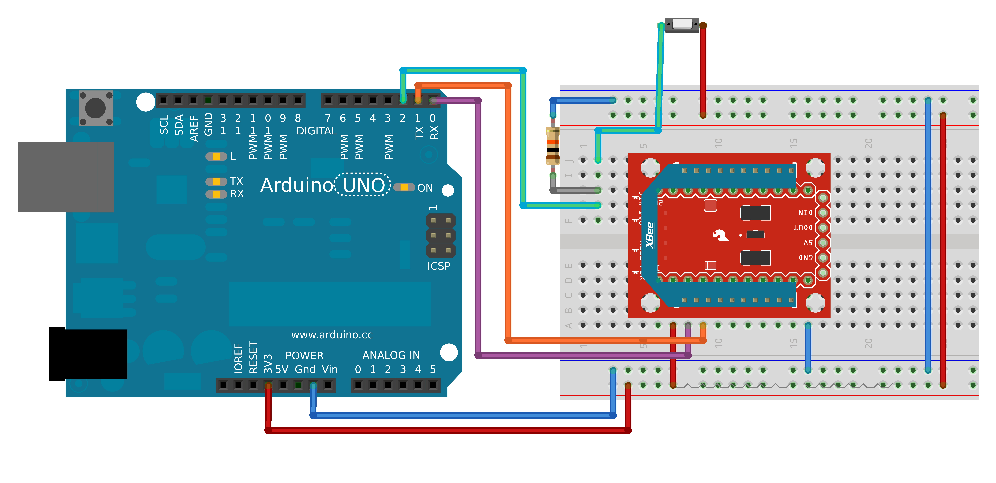
\includegraphics[width=\linewidth]{figures/doorbellSwitch-NEW.eps}
  \caption{Wireless doorbell: switch layout
  \label{fig:wirelessDoorbellSwitch}}
\end{figure}

\begin{figure}[htbp]
  \centering
  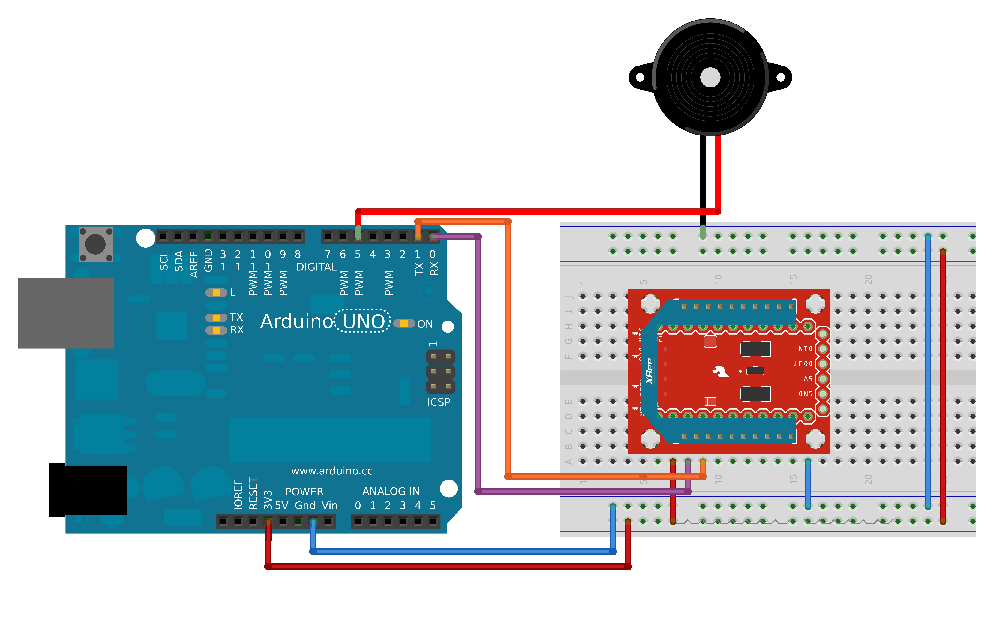
\includegraphics[width=\linewidth]{figures/doorbellBuzzer-NEW.eps}
  \caption{Wireless doorbell: buzzer layout
  \label{fig:wirelessDoorbellBuzzer}}
\end{figure}

\section{The code}\label{wirelessDoorbellCode}
\subsection{XBee code}

First, start with the coordinator. It is recommended that you attach a sticker or some kind of mark to each XBee so you will know which one is the coordinator and the router.
\begin{enumerate}
  \item Start a terminal session with the XBee. You can use any terminal application or the terminal utility in the X-CTU.
  \item To start interactive mode, type \texttt{+++} and the XBee will respond with an \texttt{OK} message. You're in!
  \item Select a PAN ID number between 0x0 and 0x(16 Fs), so there are plenty PAN IDs. Then, configure the XBee to work in this PAN ID by entering \texttt{ATID} followed by the PAN ID you selected and press enter. The XBee should respond with an \texttt{OK} message. If not, then maybe you were thrown out of command mode. Retry by issuing the \texttt{+++} command again.
  \item Because we are working with a pair of radios, this one should have as a destination address the address of the other XBee you are using. So, enter the \emph{high} part of the other XBee destination address by typing \texttt{ATDH 0013A200}.
  \item Then, enter the \emph{low} part of the destination address by typing \texttt{ATDL} followed by your other XBee's lower address.
  \item Write your configuration by issuing \texttt{ATWR} and pressing enter.
\end{enumerate}

Repeat this same process with your other XBee. Remember that:

\begin{itemize}
  \item You will be thrown out of command mode after 10 seconds of inactivity. To re-enter enter the \texttt{+++} command and wait for the \texttt{OK} response.
  \item The destination addresses are those of the other XBee! This is a frequent mistake.
  \item After making changes, always save them by entering the \texttt{ATWR} command.
\end{itemize}

\subsection{The Arduino code}
\subsubsection{The button Arduino}
This code corresponds with the button side of the example.
\\
{\color{red}{There's a trap!}}: when uploading programs to your Arduino, disconnect the digital pin 0 (RX) and then reconnect it after the loading is completed. Otherwise you will receive an error.

\begin{lstlisting} [caption = {Configuring the Arduino of the buttom side of the example.}, language = C, label = {code:wirelessDoorbellButton}, numbers = left, escapeinside={@}{@}] 
int BUTTON = 2;
void setup() { 
	pinMode(BUTTON, INPUT); 
	Serial.begin(9600);
}
void loop() {
// send a capital D over the serial port if the button is pressed
	if (digitalRead(BUTTON) == HIGH) { 
		Serial.print('D');
		delay(10); // prevents overwhelming the serial port 
	}
}
\end{lstlisting}

\subsubsection{The buzzer Arduino}
This Arduino will receive a signal when the button is pressed and will ring the buzzer.

\begin{lstlisting} [caption = {Configuring the Arduino of the buzzer side of the example.}, language = C, label = {code:wirelessDoorbellBuzzer}, numbers = left, escapeinside={@}{@}]
int BELL = 5;
void setup() { 
	pinMode(BELL, OUTPUT); 
	Serial.begin(9600);
}
void loop() {
	// look for a capital D over the serial port and ring the bell if found 
	if (Serial.available() > 0) {
		if (Serial.read() == 'D'){ 
		//ring the bell briefly 
			digitalWrite(BELL, HIGH); 
			delay(10); 
			digitalWrite(BELL, LOW);
		}		 
	}
}
\end{lstlisting}

\section{Next Steps}
\begin{itemize}
\item The Arduino on the buzzer side can send a confirmation to the Arduino on the push-button side.
This confirmation means that the initial message has been received and the buzzer is buzzing.
Include an additional LED on the switch side that lights up when this confirmation is received.
Now try the doorbell again.
Confirm that the LED lights up when the button is pushed.
Finally, disconnect the Arduino on the buzzer side and try to push the button again.
There should be no sound and no light.
\item Make a more sophisticated doorbell.
Include an LED on the buzzer side.
When the button is pressed, the LED lights up.
When the button is pressed for longer than one second, the buzzer buzzes.
\item The challenge. The buzzer side has a light sensor. During the day, it behaves as a regular buzzer.
If it is dark, it lights up a LED and sounds the buzzer only when the button has been pressed for over three seconds.
The buzzer side sends feedback to the button side.
The button side will blink a LED while the remote LED is on and turn on a steady LED when the buzzer is being sounded.

\end{itemize}





